%!TEX root = ../template.tex
%%%%%%%%%%%%%%%%%%%%%%%%%%%%%%%%%%%%%%%%%%%%%%%%%%%%%%%%%%%%%%%%%%%
%% chapter4.tex
%% NOVA thesis document file
%%
%% Chapter with introduction
%%%%%%%%%%%%%%%%%%%%%%%%%%%%%%%%%%%%%%%%%%%%%%%%%%%%%%%%%%%%%%%%%%%

\typeout{NT FILE chapter5.tex}%

\chapter{Spectral analysis}

Now that the theoretical spectrum has been simulated, it is time to analyze the evolution of the emission lines with the change in the beam energy. Results will then be compared with a recent work by Y. Ito ?? where measurements of Copper's x-ray transitions were taken for



\section{Result analysis}

For the purpose of peak analysis of the $K_{\alpha}$ spectrum, it is common practice to employ either four Lorentzian profile, or two asymmetrical ones. The latter approach was the one applied for this study.


In order to compute the asymmetrical Lorentzian profile, an asymmetry parameter, $\alpha$, was incorporated:

\begin{equation}
    L_{\text{assim}}(E-E_{i,f},\Gamma_{i,f},\sigma,\alpha)=\frac{I_{i,f}}{2\pi}\frac{\Gamma_{i,f}}{\qty(\frac{E-E_{i_f}}{\alpha\cdot \text{sign}\qty(E-E_{i_f})+1})^2+\qty(\frac{\Gamma_{i,f}}{2})^2}
\end{equation}

The influence of the calculated excitations, namely to orbital $5p$, will now be noticed in the evolution of the parameters, resulting, in some cases, in extremely non-linear parameter progression.
\subsection{Centroid energy}

For the $K_{\alpha_1}$ line, a very noticeable energy shift of around $0.5\ \si{\electronvolt}$ is observed at the second $4p$ resonance-dominated zone. Once again, poor numerical convergence may be the cause of this.

On the case of the $K_{\alpha_2}$ line, the results are less anomalous, as there is a steady rise of the centroid energy, with the influence of different excited states being noted as sudden bumps and lows.

Both spectral line energies are lower on the pre-ionization region, and saturate for beam energy values over the K edge, with $K_{\alpha_1}$ possessing an energy of $\qty(8047.093\pm0.002)\ \si{\electronvolt}$ and $K_{\alpha_2}$ of $\qty(8026.683\pm0.004)\ \si{\electronvolt}$   at $E_{\text{beam}}=8970\ \si{\electronvolt}$, and rising to $\qty(8047.12926 \pm 0.00001)\ \si{\electronvolt}$ and $\qty(8027.05247 \pm 0.00002)\ \si{\electronvolt}$, respectively, for the post-ionization region.

Figure~\ref{fig:centroid} contains the whole evolution of the centroid parameters as well as indications for the major excitation contributions.

\begin{figure}[h!]
    \centering
    \begin{tikzpicture}
        \node at (0,0){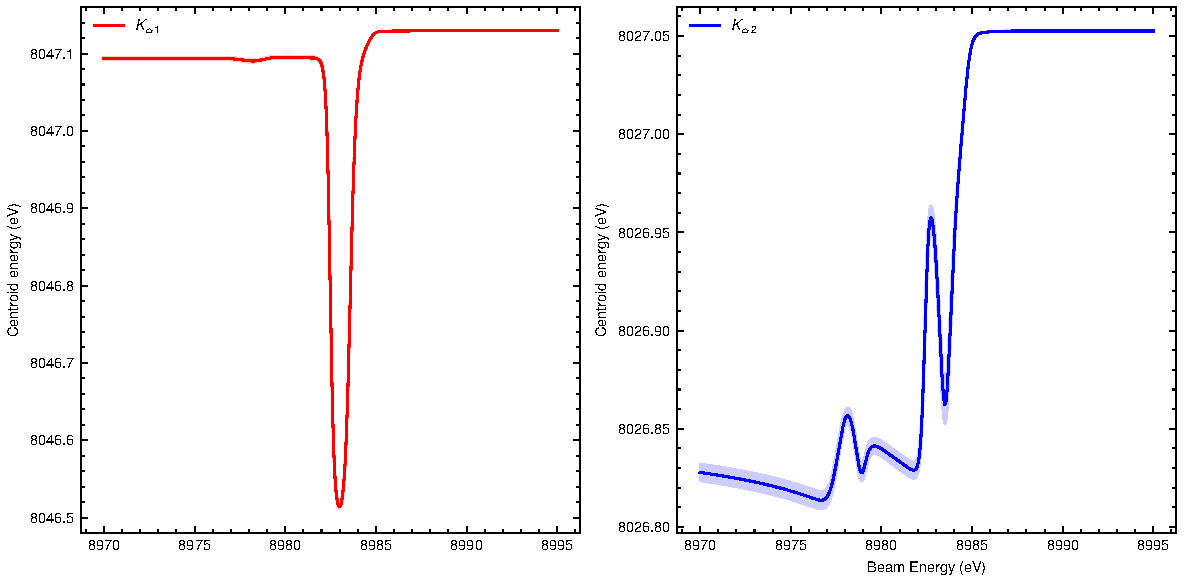
\includegraphics[width=\linewidth]{Chapters/Figures/Chapter5/assym_centroids.pdf}};
        \draw[-stealth] (2,0) node[anchor=south]{$4s$} -- (3,-1.5);
        \draw[-stealth] (5,-2) node[anchor=west]{$4p$} -- (3.7,-2);
        \draw[-stealth] (6,1) node[anchor=west]{$5p$} -- (4.3,1);
        
        \draw[-stealth] (-1,-2.5) node[anchor=west]{$4p$} -- (-3,-2.5);
    \end{tikzpicture}
    \caption{Evolution of centroid parameter as a function of the beam energy. The bands colored bands include the parameter fitting errors.}\label{fig:centroid}
\end{figure}

\subsection{Energy width}

Both $K_{\alpha}$ transitions present an energy width value of around $2.2\ \si{\electronvolt}$ for the post-ionization region ($\qty(2.25137\pm 0.00003)\ \si{\electronvolt}$ and $\qty(2.21834\pm 0.00006)\ \si{\electronvolt}$ for $K_{\alpha_1}$ and $K_{\alpha_2}$, respectively). Both present higher values than these for the excitation-dominated region, with $K_{\alpha_2}$ being wider than $K_{\alpha_1}$.
%With the increase on the beam energy, the ratio between the two widths tends for values closer to one (Figure).\todo{comparar com os resultados do Ito}


\begin{figure}[h!]
    \centering
    \begin{tikzpicture}
        \node at (0,0){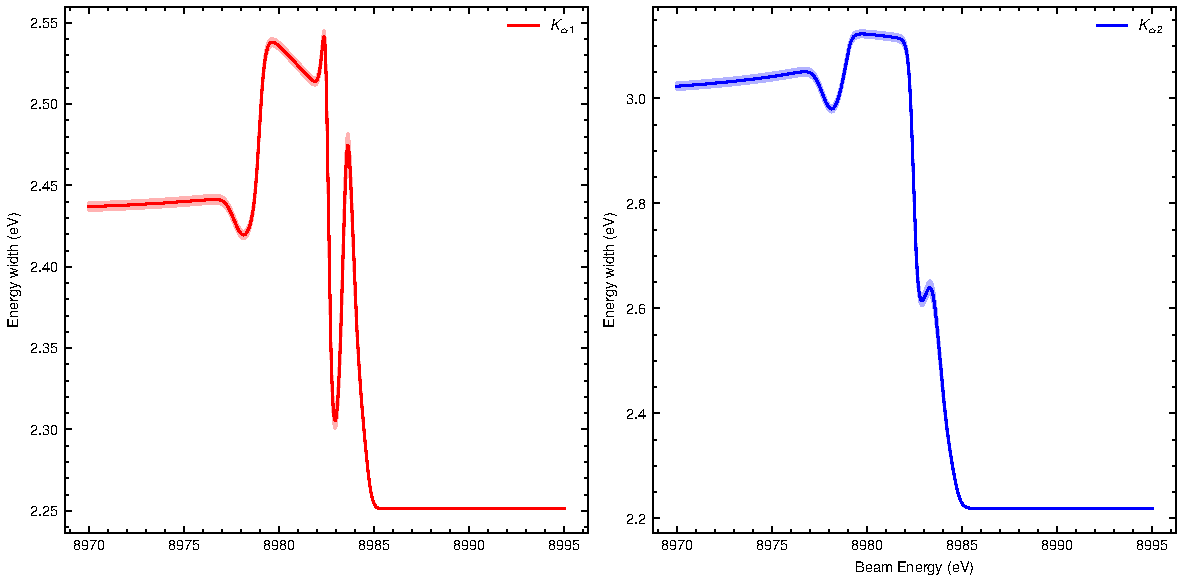
\includegraphics[width=\linewidth]{Chapters/Figures/Chapter5/assym_widths.pdf}};
        \draw[-stealth] (-5,0) node[anchor=north]{$4s$} -- (-4.5,0.5);
        \draw[-stealth] (3,1) node[anchor=north]{$4s$} -- (3,2.2);
        \draw[-stealth] (-4,4) node[anchor=south]{$4p$} -- (-4,3.2);
        \draw[-stealth] (-4,4) node[anchor=south]{$4p$} -- (-3.5,3.2);
        \draw[-stealth] (3.5,4) node[anchor=south]{$4p$} -- (3.5,3.4);
        \draw[-stealth] (-1,2) node[anchor=west]{$5p$} -- (-3,2);
        \draw[-stealth] (6,0) node[anchor=west]{$5p$} -- (4.5,0);
    \end{tikzpicture}
    
    \caption{Evolution of transition width as a function of the beam energy.}\label{fig:width}
\end{figure}

The fact the transition widths  for the photoexcitation region present a higher value  than for the standard $K_{\alpha}$ transitions for ionized Copper could be easily explained by the increase in the amount of Auger decay channels due to the presence of a lesser bound electron, whose transitions will lead to greater level widths.
% \begin{figure}
    % \centering
    % 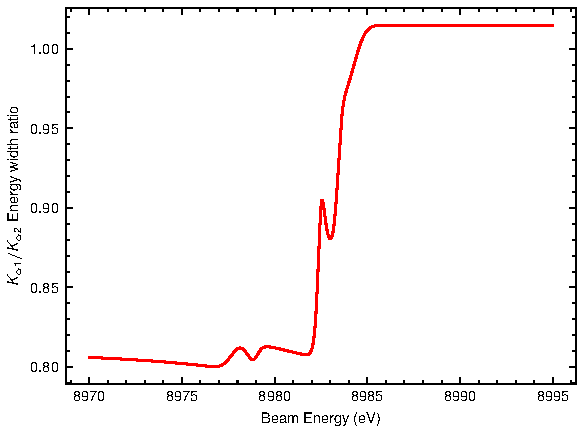
\includegraphics[width=.6\linewidth]{Chapters/Figures/Chapter5/assym_ratio_width.pdf}
    % \caption{Evolution of the ratio between transition widths.}\label{fig:ratio_width}
% \end{figure}


\subsection{Spectral intensity}

The main takeaway point from this parameter is the growth is the immense evolution of the spectral intensity. From the lowest simulated beam energy to the post-ionization regime, the spectral intensity for both lines grows by 6 orders of magnitude. Only decays from $4p$ excited levels seem to influence significatively the spectral intensity, as can be noticed by the increase in intensity on Figure~??.

In addition, from the same figure, it can also be concluded that the ratio between $K_{\alpha_1}$ and $K_{\alpha_2}$ intensities, while it is about the same for most of the surveyed energies, it rapidly oscillates near the $5p$ and higher excitation energy resonances, stabilizing once again for higher energies, where ionization predominates.

\begin{figure}
    \centering
    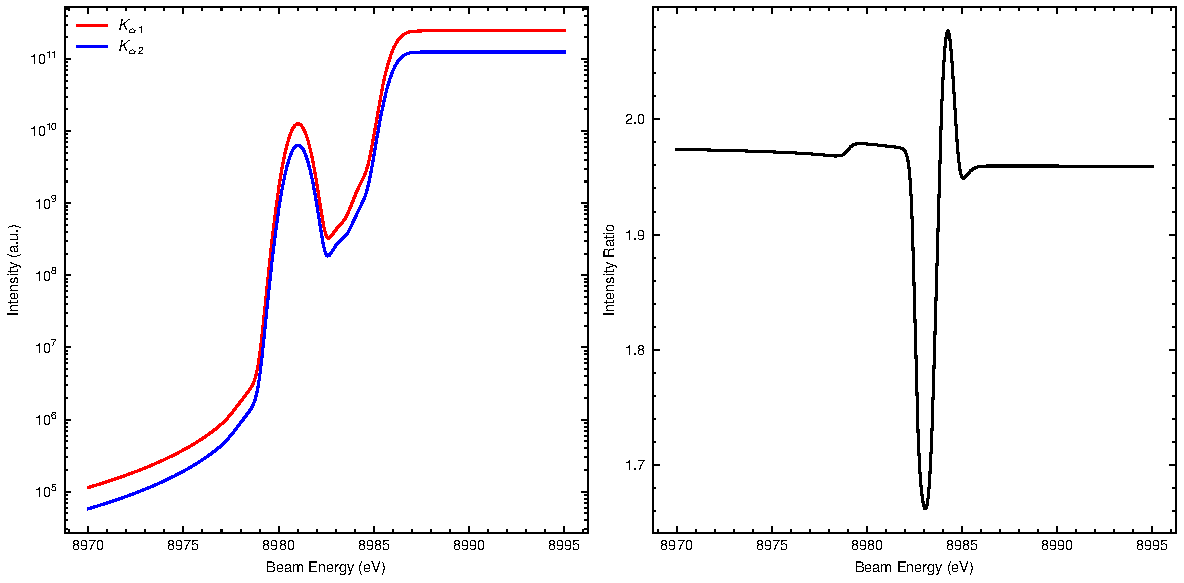
\includegraphics[width=\linewidth]{Chapters/Figures/Chapter5/assym_intensities.pdf}
    \caption{Evolution of the spectral intensity and intensity ratio.}\label{fig:intensity}
\end{figure}
\subsection{Asymmetry index}

For the model used, a negative value for the asymmetry index indicates a skewness to lower energies, while a positive for higher energies.

Figure~\ref{fig:index} shows the evolution of this parameter for both spectral lines.
While the $K_{\alpha_2}$ presents a constant left-skewness up until the ionization region, $K_{\alpha_1}$ presents as symmetric up until the second $4p$ excitation area, where it acquires a positive skewness factor, which consecutively drops when entering the area where the $5p$ excitation dominates. Both lines go back turn symmetric ($\alpha=0$) when the ionization region is reached.

\begin{figure}
    \centering
    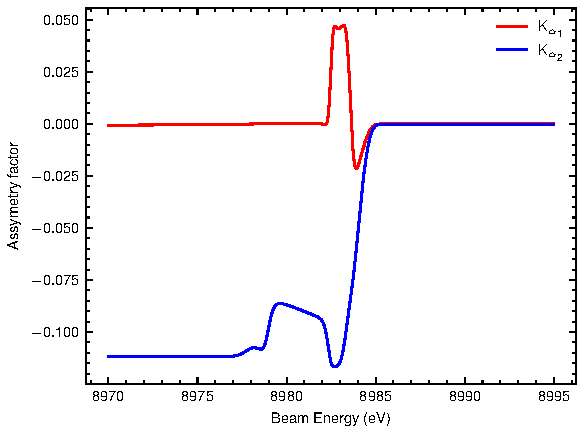
\includegraphics[width=.6\linewidth]{Chapters/Figures/Chapter5/assym_index.pdf}
    \caption{Evolution of asymmetry index.}\label{fig:index}
\end{figure}




\section{Comparison with experimental results}

It is unfortunate that not many of experiments have been run for exploring the phenomenon of photoexcitations of K-shell electrons and the consequent decays. Due to the low spectral intensity, and the fine structure of the resonances, exploring the photoexcitation effect can be quite challenging.

In a recent work by Y. Ito \todo{cite}, near-threshold beam energies produced in a synchrotron line have been used to probe a Copper target. The consequent emitted radiation was then measured by the means of a Double Crystal Spectrometer. The wavelength dispersive nature of this apparatus allows for very precise filtering of the measured energy, allowing for experimental resolutions lower than $1\ \si{\electronvolt}$. The beam energy was tuned from values as low as $8978\ \si{\electronvolt}$, which falls under the theoretical excitation-dominated region, up to post-ionization threshold values. In this experimental setup, however, the measured $K$-edge presented a value of $8980.06\ \si{\electronvolt}$, so only a small portion of the measured spectrum can be of interest.

The $K_{\alpha}$ lines were consequently measured and fitted with Lorentzian profiles. Figure ?? shows the parameter evolution of the measured spectrum.


\begin{figure}
    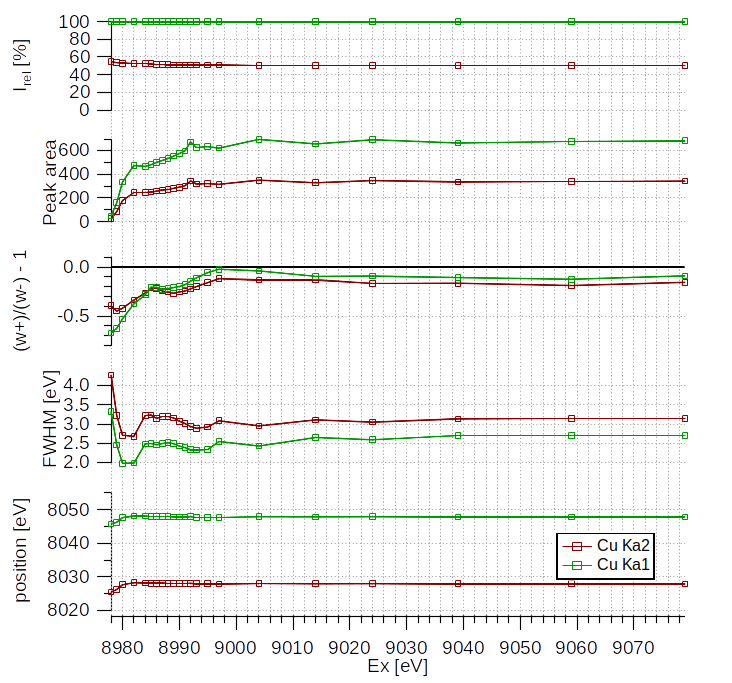
\includegraphics[width=\linewidth]{Chapters/Figures/Chapter5/ito.png}
    \caption{Components of the Lorentzian profiles employed in the fitting of the $K_{\alpha}$ spectrum. From ??.}\label{fig:ito}
\end{figure}


The main takeaway points for comparison between the calculated theoretical spectrum and the measured experimental one, is that both present larger widths for bellow-ionization threshold energies.




% There have, however, some x-ray absorption studies been performed for energies near the K-edge.

% In this case, the absorption is increasing with respect to the beam energy, with some possible resonant structures evident.

% \todo{meter figura}




On the emission spectrum, measurements have been performed for near K-edge beam energies.